\documentclass[12pt,oneside,a4paper]{article}
\usepackage{tikz}
\usetikzlibrary{arrows.meta,arrows}
\author{Siberia怒风}
\begin{document}
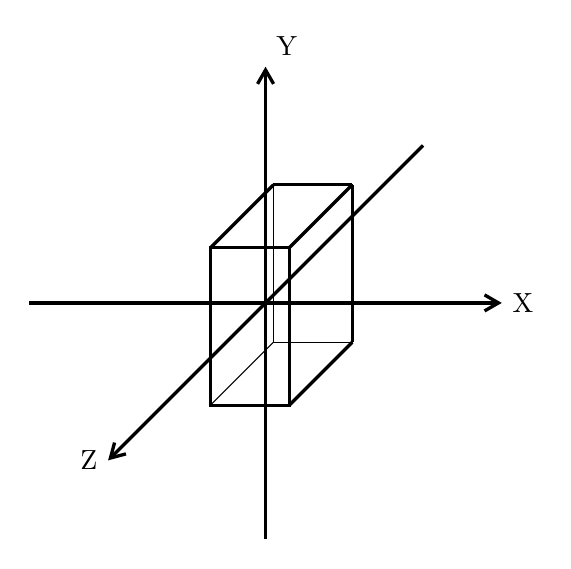
\begin{tikzpicture}
[>={Straight Barb[angle=60:1pt 4]},
myarrow/.style={
decoration={
markings,
mark=at position 0.5 with {\arrow {Straight Barb}};}
postaction = decorate}]
  \draw [->, very thick](-3,0) -- (3,0) node[right]{X};
  \draw [->, very thick](0,-3) -- (0,3) node[above right]{Y};
  \draw [->, very thick](2,2) -- (-2,-2) node[left]{Z};
  \draw [very thick] (-0.7,-1.3) rectangle (0.3,0.7);
  \draw (0.1,-0.5) rectangle (1.1,1.5);
  \draw [very thick] (-0.7,0.7) -- (0.1,1.5);
  \draw [very thick] (0.3,0.7) -- (1.1,1.5);
  \draw (-0.7,-1.3) -- (0.1,-0.5);
  \draw (0.1,-0.5) -- (0.1,1.5);
  \draw [very thick] (0.3,-1.3) -- (1.1,-0.5);
  \draw [very thick] (0.1,1.5) -- (1.1,1.5);
  \draw [very thick] (1.1,-0.5) -- (1.1,1.5);
\end{tikzpicture}
\end{document}